\documentclass[journal, a4paper]{IEEEtran}

\usepackage{algorithm}
\usepackage{algpseudocode}

\usepackage{graphicx}
\usepackage{url}  
\usepackage{amsmath}
\usepackage{hyperref}
\usepackage{xcolor}

\graphicspath{ {img/} }
\hypersetup{
  colorlinks=true,
  linkcolor=blue!50!red,
  urlcolor=blue!70!black
}

\begin{document}
\title{C++ Project - Solving Kakuro}
\author{
	Elie ABI HANNA DAHER and Bilal EL CHAMI \\ 
	GitHub repository : \href{https://github.com/elieahd/kakuro}{github.com/elieahd/kakuro}
}
\markboth{Paris Dauphine University}{}
\maketitle

\begin{abstract}
	This document illustrate the work done for an academic project that consists of solving a Kakuro Grid as a contraint satisfaction problem (CSP) in C++.
\end{abstract}

\section{Introduction}
 Kakuro consists in filling a grid with numbers that sum up to a certain values for each column and row. Each cell needs to be filled with a value between 1 and 9.\\
 The following example represents a 5x5 grid where the sum of each row has to be 15 and the sum of each column has to be 15.
\begin{figure}[h!]
    	 \begin{center}
		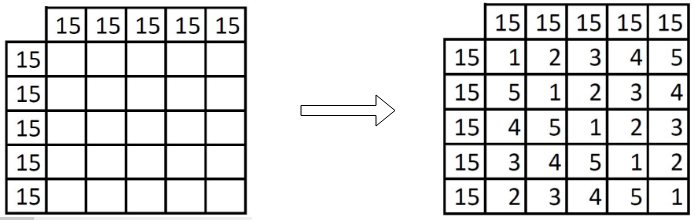
\includegraphics[width=\columnwidth]{example_kakuro.png}
  		\caption{Example of solving a 5x5 kakuro gird}
		\label{fig:example_kakuro}
    	 \end{center}
\end{figure}

\section{Implementation}
In our project we created 4 classes: $Position$, $Cell$, $Grid$ and $Kakuro$. The $Cell$ class is represented by a value and a $Position$. The $Grid$ contain a list of $Cell$. Finally the $Kakuro$ contains the $Grid$ with all the possible value that a $Cel$l can have and the target sum of rows and columns. $Kakuro$ class contains the implemented algorithm: Forward Checking and Iterative Sampling and Iterative Meta Monte Carlo. \\

\subsection{Grid}
The initial grid of the kakuro will be present in a file, which will contain the possible values of a cell and the target sum of each column and row. We have tested our project in 5 different grids with different sizes between 4x4 and 6x6 grid. You can find the different girds under the folder \textit{grids} in the GitHub repository.

\subsection{Choosing variable}
While solving the Kakuro grid, we have decided to choose the variable (Cell) tha--t has the smallest domain size. In both algorithm, forward checking and monte carlo, we have implemented the same logic regarding the choice of variable.

\section{Search Algorithms}
We implemented two algorithms: Forward Checking and Monte Carlo.
\subsection{Forward Checking}
This algorithm consist in reducing the domain of each variable not assigned. Each time a value is assigned to a cell, the value is removed from the domain of the cell in the same row and column. To check if we need to backtrack, two conditions are evaluated, the first one is making sure that all the unassigned Cell don't have an empty domain and the other condition is making sure that the grid is consistent which will evalute the row or column where all the cell are assigned and make sure that they match the target sum.

\subsection{Iterative Sampling}
This algorithm consist in assiging a random value for a Cell, and in case of inconsistency in the grid or in case of an empty domain for an unassigned cell we will reinitialize the grid and restart the algorithm. 

\subsection{Iterative Meta Monte Carlo}
This algorithm consist in assiging a random value for a Cell, and in case of inconsistency in the grid or in case of an empty domain for an unassigned cell we will reinitialize the grid and restart the algorithm. 

\section{Experimentals - Simulation}
In order to test the perfomance of our algorithm, we runned several grids 100 times and calculated the estimated time to solve the kakuro grid using both algorithm. 

    \begin{table}[!hbt]
        \begin{center}
        \caption{Simulation}
        \label{tab:simParameters}
        \begin{tabular}{|c|c|c|c|}
            \hline
           Grids & Forward Checking &  Iterative Sampling & Meta Monte Carlo \\
            \hline
           2x2 & $0.02$ s  &  $ 0.019 $ s   &  $ 0.019 $ s  \\
            \hline
           3x3 & $0.021$ s  &  $ 0.02 $ s &  $ 0.019 $ s    \\
            \hline
           4x4 & $ 2.804  $ s  &  $ 0 $ s  &  $ 0.019 $ s   \\
            \hline
           5x5 & $5.02$ s  &  $ 0 $ s &  $ 0.019 $ s    \\
            \hline
           6x6 & $ 10,152.1$ s  &  $ 0 $ s  &  $ 0.019 $ s   \\
            \hline
        \end{tabular}
        \end{center}
    \end{table}
The time of execution of both algorithm are both very dependant from several criteria. The first one is the size of the grid, the second criteria is the target sum the final criteria is possible values.
The forward checking algorithm is more optimal and more efficient than the monte carlo algorithm. \\
We could have tested both algorithm together by modifing the forward checking algorithm to take a random value instead of having to iterate through the values.

\begin{thebibliography}{5}
    \bibitem{MonteCarloKakuro} 
    T.~Cazenave. {\em Monte-Carlo Kakuro}

   \bibitem{WikiKakuro} 
   Wikipedia page on {\em Kakuro}. [Online]. \\ Available:  \url{ https://en.wikipedia.org/wiki/Kakuro}

   \bibitem{WikiCSP} 
   Wikipedia page on {\em CSP }. [Online]. \\ Available:  \url{https://en.wikipedia.org/wiki/Constraint_satisfaction_problem}

   \bibitem{WikiBacktracking} 
   Wikipedia page on {\em Backtracking algorithm}. [Online]. \\ Available:  \url{https://en.wikipedia.org/wiki/Look-ahead_(backtracking)}

\end{thebibliography}

\end{document}